\section{Simulation Analysis }
\label{sec:simulation}

\subsection{AC/DC converter graphs}

In this section we evaluated the AC/DC converter proposed. To simplify the calculations for NGSpice, we have decided to use the circuit \ref{fig:SIM_ANG}, since using the ideal model for the ransformer was causing NGSpice to slow down significantly.
In order to analise the circuit after the transiant period, we have chosen $t \in \left \[ 0.010 ; 200 \left \[$ ms.

The graphs for NGSpice are displayed here, alongside the table with the required elements:

\begin{figure}[h] \centering
\vspace{-3cm}
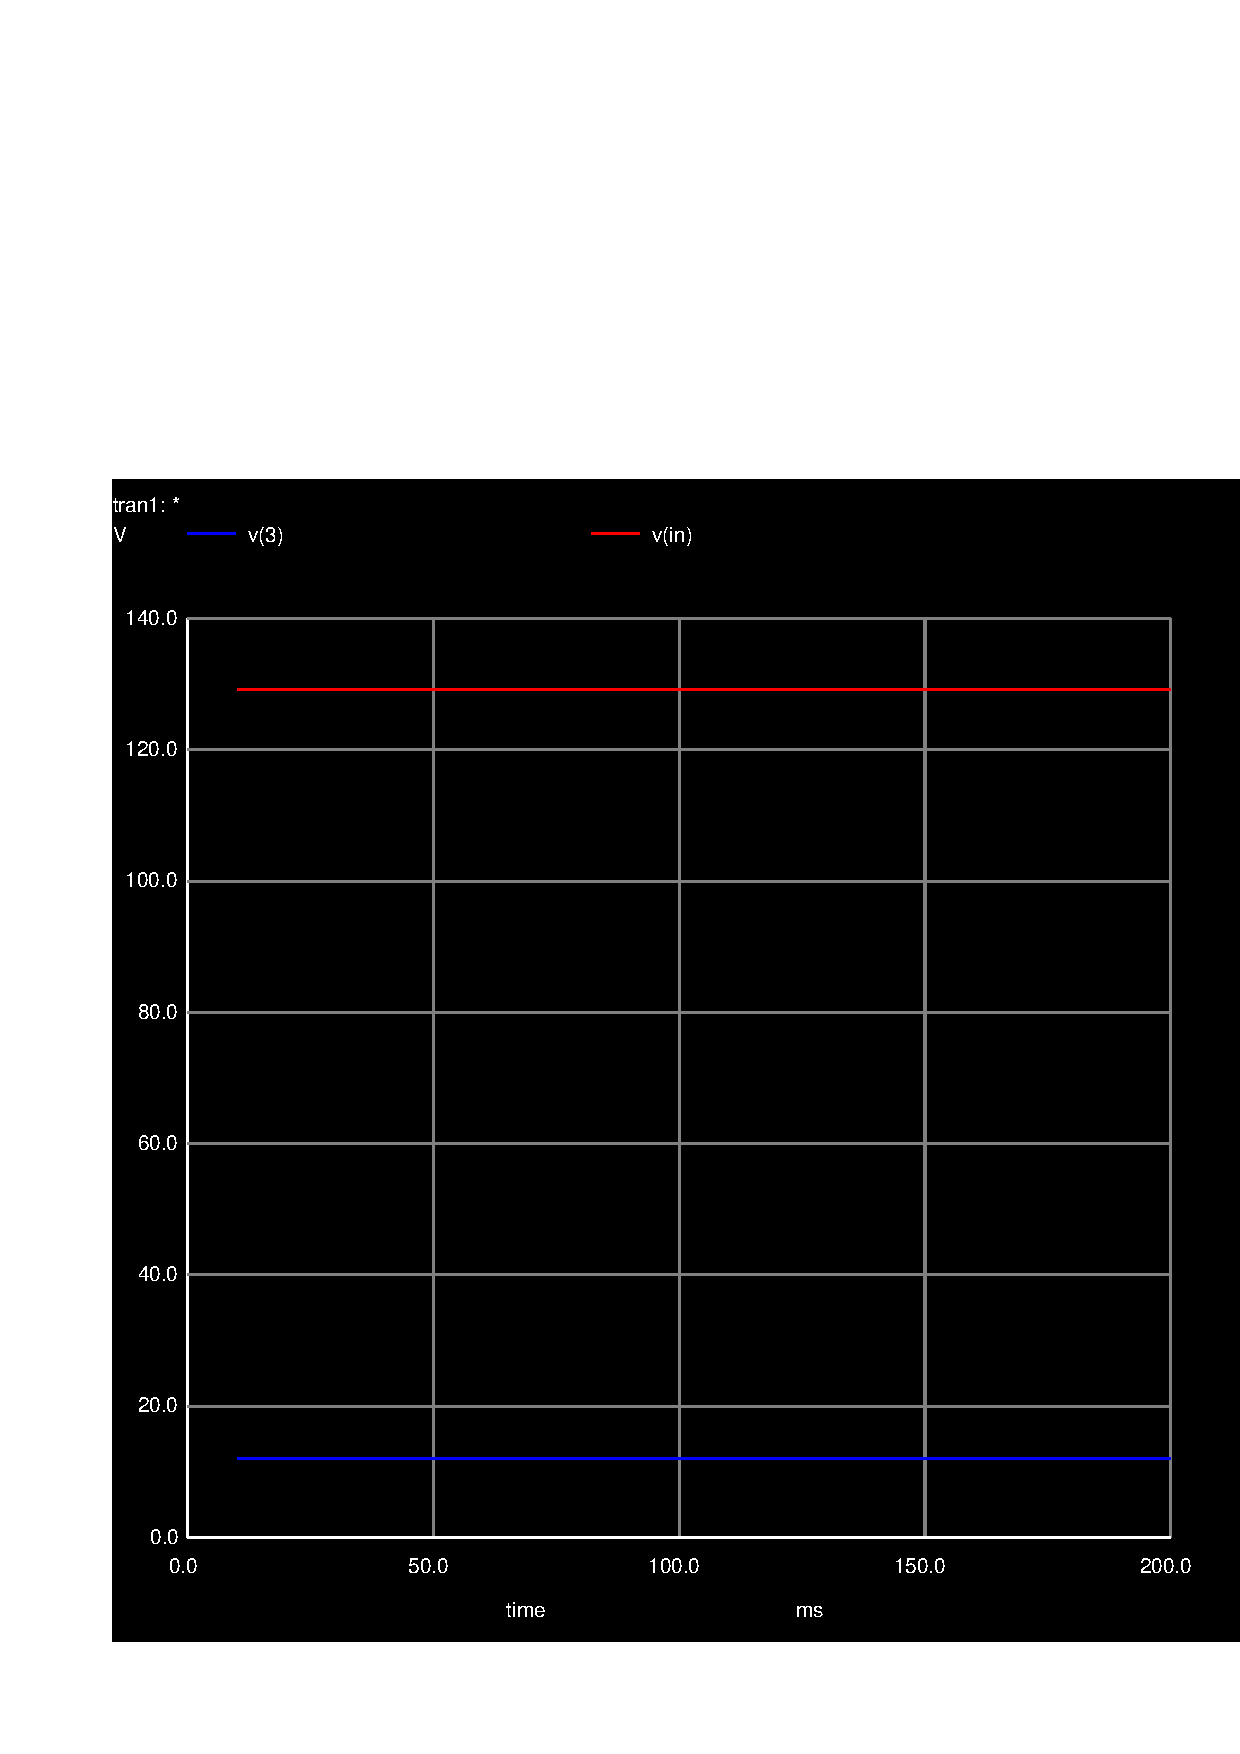
\includegraphics[height=10cm]{../sim/trans4.pdf}
\caption{$v_3(t)$ ($v_{OUT}(t)$) and $v_{IN}$ ($v_{Envelope}(t)$)}
\label{fig:SIM_FULL_RES}
\end{figure}

\begin{figure}[h] \centering
\vspace{-3cm}
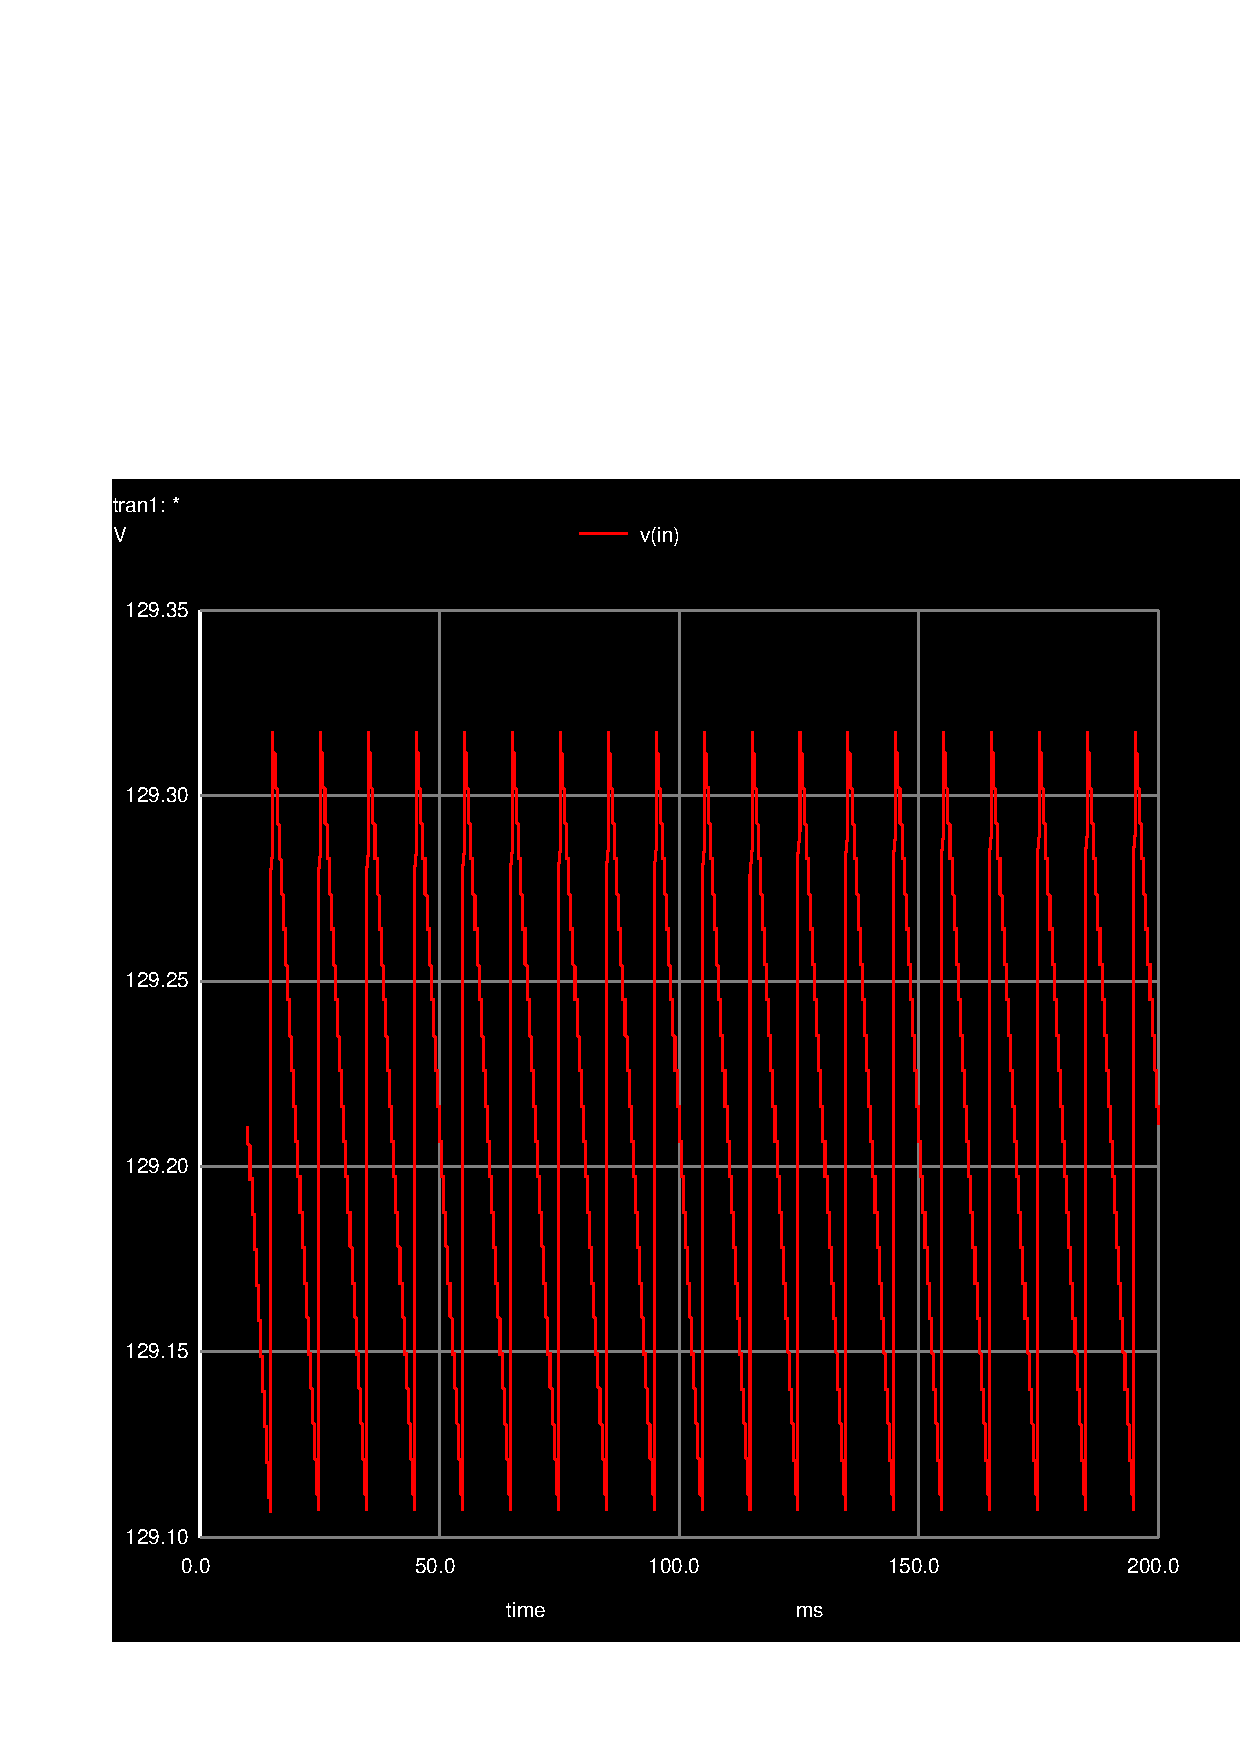
\includegraphics[height=10cm]{../sim/trans41.pdf}
\caption{$v_{IN}(t)$ ($v_{Envelope}(t)$)}
\label{fig:SIM_FULL_ENV}
\end{figure}

\begin{figure}[h] \centering
\vspace{-3cm}
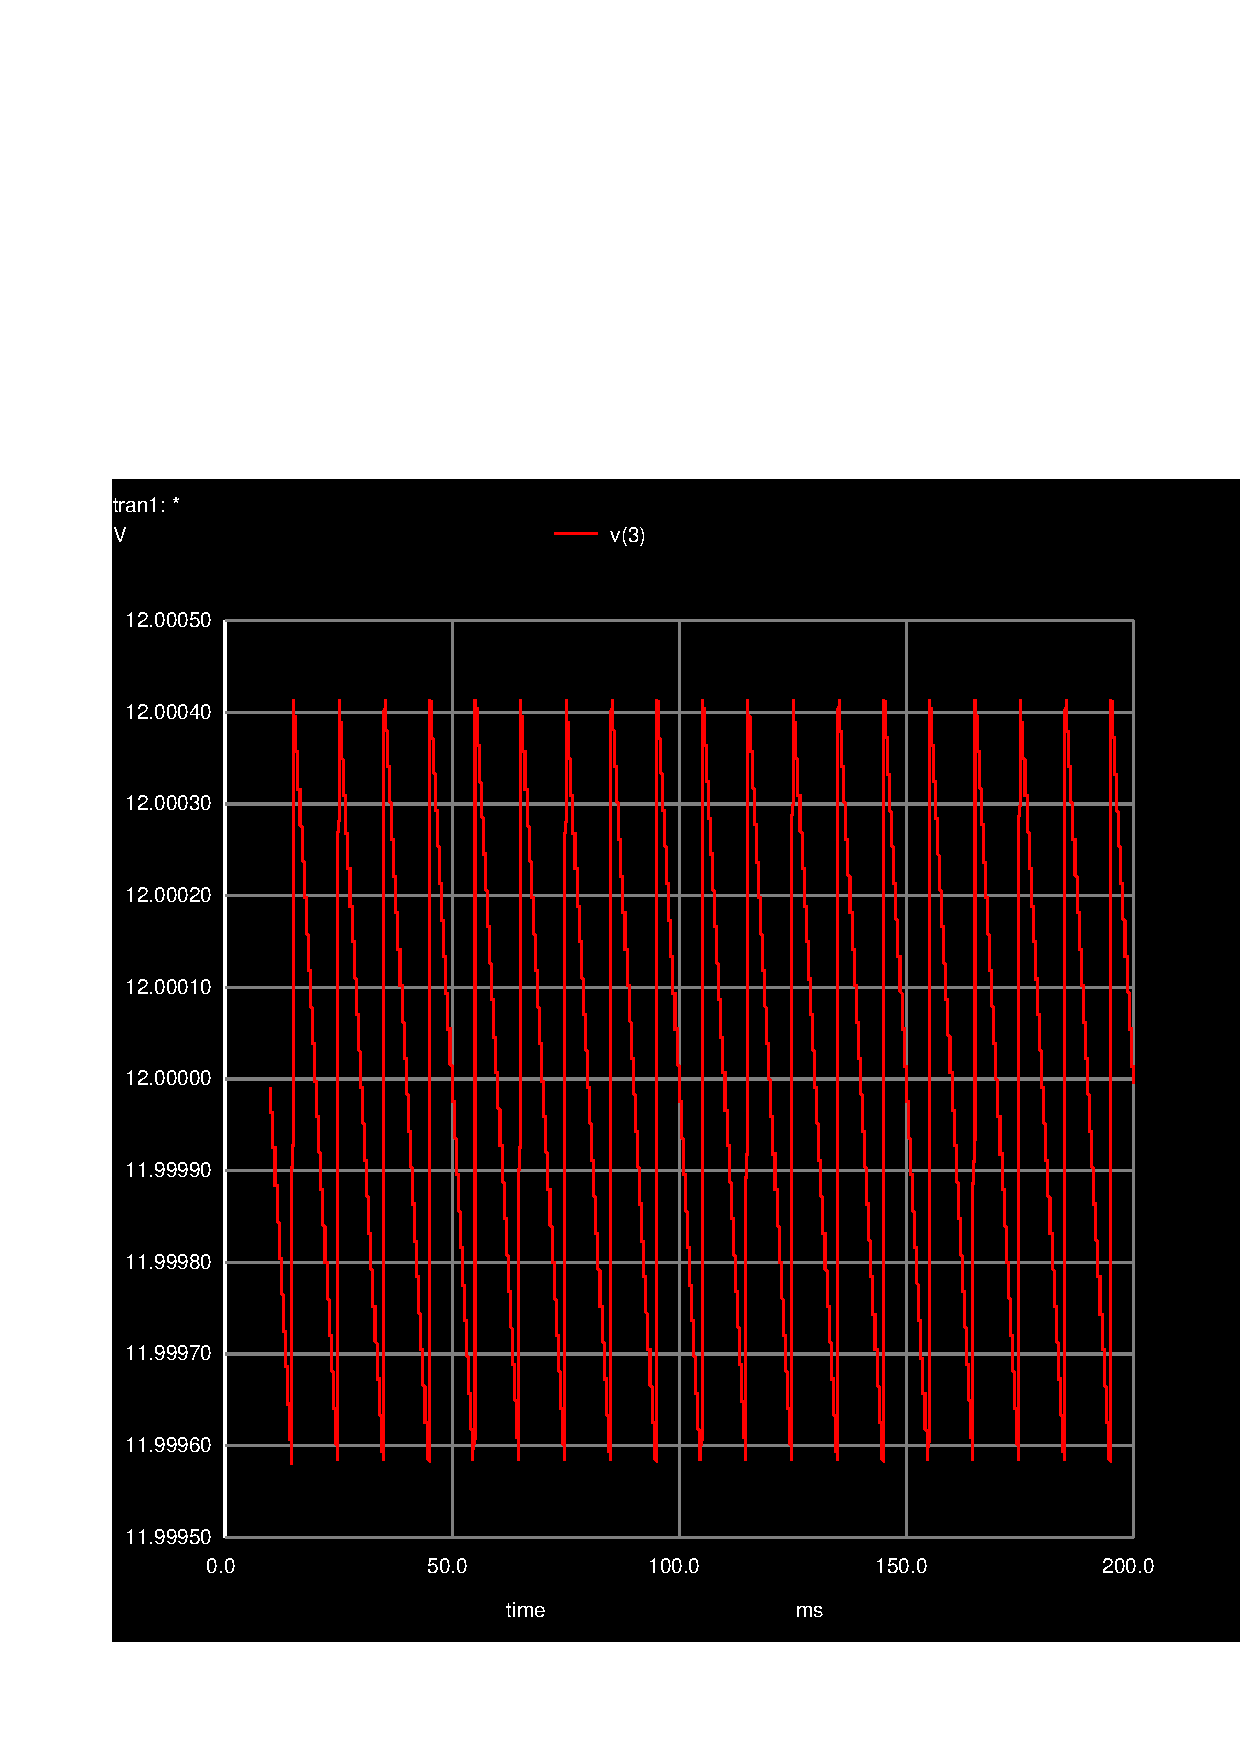
\includegraphics[height=10cm]{../sim/trans42.pdf}
\caption{$v_{3}(t)$ ($v_{OUT}(t)$)}
\label{fig:SIM_FULL_OUT}
\end{figure}

Table~\ref{tab:SIM_RESULTADOS} shows the simulated operating point results for the circuit under analysis.
%Colocar a tabela 
\begin{table}[h]
  \centering
  \begin{tabular}{|l|r|}
    \hline    
    {\bf Name} & {\bf Value [A or V]} \\ \hline
    n & 0.56882248\\ \hline
cost & 302.2\\ \hline
mean(v(3))-12 & 5.094465e-07\\ \hline
vecmax(v(3))-vecmin(v(3)) & 8.328428e-04\\ \hline
1 / (abs(mean(v(3))-12) + vecmax(v(3))-vecmin(v(3)) + 1u) / (150+150+(18 + 4)*.1) & 3.966031e+00\\ \hline

  \end{tabular}
  \caption{Operating point for $t<0$. A variable preceded by £ is of type {\it cost} and expressed in Unit of Cost; other variables are of type {\it voltage} and expressed in Volt. Merit as it's units in {\it per voltage per cost} and expressed in Volt$^{-1}$UC$^{-1}$ }
  \label{tab:SIM_RESULTADOS}
\end{table}

Compared to the theoretical analysis the simulation showed practically identical results, except for a small divergence in the last decimal place that probably occurs when Ngspice rounds the numbers. Thus, the maximum relative error is $10^{-5}$. It is worth mentioning that Ngspice software also uses the same mathematical methods as octave to find results, hence, this result was already expected.


When comparing the graphics obtained in Ngspice and Octave, the similarity between the results is noticeable and small differences can be explained by approximation errors.



